%%%%%%%%%%%%%%%%%%%%%%%%%%%%%%%%%%%%%%%%%
% Short Sectioned Assignment LaTeX Template Version 1.0 (5/5/12)
% This template has been downloaded from: http://www.LaTeXTemplates.com
% Original author:  Frits Wenneker (http://www.howtotex.com)
% License: CC BY-NC-SA 3.0 (http://creativecommons.org/licenses/by-nc-sa/3.0/)
%%%%%%%%%%%%%%%%%%%%%%%%%%%%%%%%%%%%%%%%%

%----------------------------------------------------------------------------------------
%	PACKAGES AND OTHER DOCUMENT CONFIGURATIONS
%----------------------------------------------------------------------------------------

\documentclass[paper=a4, fontsize=11pt]{scrartcl} % A4 paper and 11pt font size

% ---- Entrada y salida de texto -----

\usepackage[T1]{fontenc} % Use 8-bit encoding that has 256 glyphs
\usepackage[utf8]{inputenc}
%\usepackage{fourier} % Use the Adobe Utopia font for the document - comment this line to return to the LaTeX default

% ---- Idioma --------

\usepackage[spanish, es-tabla]{babel} % Selecciona el español para palabras introducidas automáticamente, p.ej. "septiembre" en la fecha y especifica que se use la palabra Tabla en vez de Cuadro

\usepackage{eurosym}
\usepackage{enumitem}

% ---- Otros paquetes ----

\usepackage{url} % ,href} %para incluir URLs e hipervínculos dentro del texto (aunque hay que instalar href)
\usepackage{amsmath,amsfonts,amsthm} % Math packages
%\usepackage{graphics,graphicx, floatrow} %para incluir imágenes y notas en las imágenes
\usepackage{graphics,graphicx, float} %para incluir imágenes y colocarlas

% Para hacer tablas comlejas
%\usepackage{multirow}
%\usepackage{threeparttable}

%\usepackage{sectsty} % Allows customizing section commands
%\allsectionsfont{\centering \normalfont\scshape} % Make all sections centered, the default font and small caps

\usepackage{fancyhdr} % Custom headers and footers
\pagestyle{fancyplain} % Makes all pages in the document conform to the custom headers and footers
\fancyhead{} % No page header - if you want one, create it in the same way as the footers below
\fancyfoot[L]{} % Empty left footer
\fancyfoot[C]{} % Empty center footer
\fancyfoot[R]{\thepage} % Page numbering for right footer
\renewcommand{\headrulewidth}{0pt} % Remove header underlines
\renewcommand{\footrulewidth}{0pt} % Remove footer underlines
\setlength{\headheight}{13.6pt} % Customize the height of the header

\numberwithin{equation}{section} % Number equations within sections (i.e. 1.1, 1.2, 2.1, 2.2 instead of 1, 2, 3, 4)
\numberwithin{figure}{section} % Number figures within sections (i.e. 1.1, 1.2, 2.1, 2.2 instead of 1, 2, 3, 4)
\numberwithin{table}{section} % Number tables within sections (i.e. 1.1, 1.2, 2.1, 2.2 instead of 1, 2, 3, 4)

\setlength\parindent{0pt} % Removes all indentation from paragraphs - comment this line for an assignment with lots of text

\newcommand{\horrule}[1]{\rule{\linewidth}{#1}} % Create horizontal rule command with 1 argument of height

\usepackage{listings}
\usepackage{hyperref}

\hypersetup{
	bookmarks=true,         % show bookmarks bar?
	unicode=false,          % non-Latin characters in Acrobat’s bookmarks
	pdftoolbar=true,        % show Acrobat’s toolbar?
	pdfmenubar=true,        % show Acrobat’s menu?
	pdffitwindow=false,     % window fit to page when opened
	pdfstartview={FitH},    % fits the width of the page to the window
	pdftitle={Practica 3 },    % title
	pdfauthor={Cristian Vélez Ruiz},     % author
	pdfsubject={ISE},   % subject of the document
	pdfnewwindow=true,      % links in new PDF window
	colorlinks=true,       % false: boxed links; true: colored links
	linkcolor=black,          % color of internal links (change box color with linkbordercolor)
	citecolor=green,        % color of links to bibliography
	filecolor=black,      % color of file links
	urlcolor=black           % color of external links
}
%----------------------------------------------------------------------------------------
%	TÍTULO Y DATOS DEL ALUMNO
%----------------------------------------------------------------------------------------

\title{	
\normalfont \normalsize 
\textsc{\textbf{Ingeniería de Servidores (2016-2017)} \\ Grado en Ingeniería Informática \\ Universidad de Granada} \\ [25pt] % Your university, school and/or department name(s)
\horrule{0.5pt} \\[0.4cm] % Thin top horizontal rule
\huge Memoria Práctica 3 \\ % The assignment title
\horrule{2pt} \\[0.5cm] % Thick bottom horizontal rule
}

\author{Cristian Vélez Ruiz} % Nombre y apellidos

\date{\normalsize\today} % Incluye la fecha actual

%----------------------------------------------------------------------------------------
% DOCUMENTO
%----------------------------------------------------------------------------------------
\begin{document}

\maketitle % Muestra el Título

\newpage %inserta un salto de página

\tableofcontents % para generar el índice de contenidos

\listoffigures

\listoftables

\newpage

%----------------------------------------------------------------------------------------
%	Cuestión 1
%----------------------------------------------------------------------------------------
\section[Cuestión 1]{a) ¿Qué archivo le permite ver qué programas se han instalado con el gestor de paquetes? 1.b) ¿Qué significan las terminaciones.	1.gz o .2.gz de los archivos en ese directorio?}

\begin{enumerate}[label=(\alph*)]
	
	\item Para poder ver los programas que se han instalado con el gestor de paquetes podemos ir al archivo \textit{/var/log/dpkg.log}, este fichero pertenece al log de dpkg \cite{dpkg}, que es la base de nuestro gestor de paquetes. 
	
	Si queremos visualizar nosotros mismos los paquetes que están instalados 
	
	Otra opción para visualizar paquetes instalados en nuestro sistema es usar la orden \textit{dpkg --get-selections}, nos muestra lo que está instalado en nuestro sistema.
	
	\item Las terminaciones de esos archivos hacen referencia a que son archivos comprimidos, se crean para ahorrar espacio en el sistema sin tener que eliminar todos los log.
	
	Cuando se va a generar un nuevo archivo comprimido se le cambia el nombre a los anteriores, por tanto el fichero mas antiguo en este caso sería el fichero .2.gz.
	
\end{enumerate}

%----------------------------------------------------------------------------------------
%	Cuestión 2
%----------------------------------------------------------------------------------------
\section[Cuestión 2]{¿Qué archivo ha de modificar para programar una tarea?Escriba la línea necesaria para ejecutar una vez al día una copia del directorio ~/codigo a ~/seguridad/\$fecha donde \$fecha es la fecha actual	(puede usar el comando date)}

Para poder programar una tarea es necesario la ayuda de cron  que es el demonio que se encarga de ir ejecutando las tareas que se definen en el crontab \cite{crontab}, para programar una tarea en el crontab usaremos \textit{crontab -e}, ya que no tenemos ningún crontab aun, en el caso de que existiera uno ya anteriormente realizaríamos lo mismo pero con \textit{crontab -l}, para no tener que eliminar lo anterior.

Nuestro script es,

\lstset{language=bash}

\begin{lstlisting}[frame=single]  
DIA=`date +"%d/%m/%y"`
mkdir -p ~/seguridad/$DIA
cp -r ~/codigo/* ~/seguridad/$DIA
\end{lstlisting}

Con eso lo que conseguimos es hacer una variable con el nombre de la nueva carpeta en formato día/mes/año y a continuación lo que hacemos es copiar lo que tenemos en el directorio código a esa carpeta.

Ahora lo que tenemos que hacer es automatizarlo para que se ejecute una vez al día, como no tenemos ningún crontab creado anteriormente lanzaremos \textit{crontab -e} y programaremos nuestro script.

\begin{figure}[H] %con el [H] le obligamos a situar aquí la figura
	\centering
	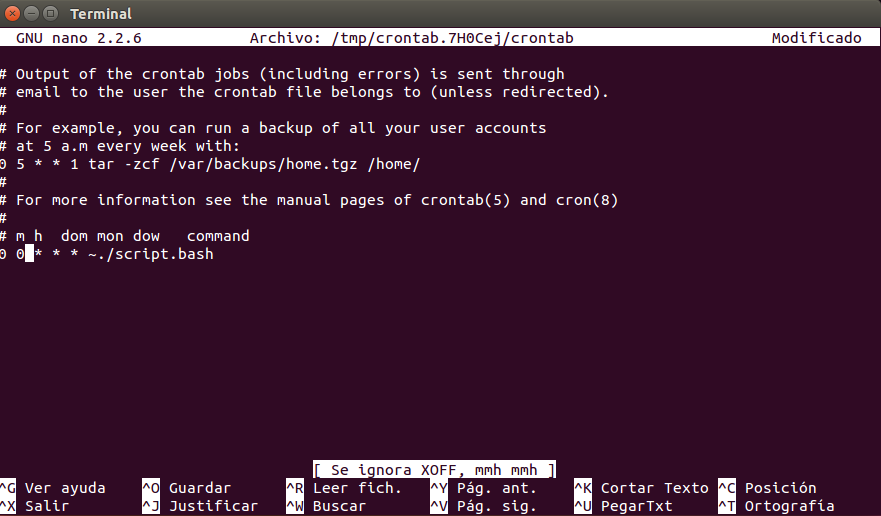
\includegraphics[scale=0.5]{pics/crontab.png}  %el parámetro scale permite agrandar o achicar la imagen. En el nombre de archivo puede especificar directorios
	\caption{Creación crontab} \label{fig:figura1}
\end{figure}

Con esa configuración le decimos que se ejecute a la hora 0 y en el minuto 0 todos los días y nos ejecute el script anterior.

Guardamos y seguidamente nos informa de que se ha creado nuestro nuevo crontab.

\begin{figure}[H] %con el [H] le obligamos a situar aquí la figura
	\centering
	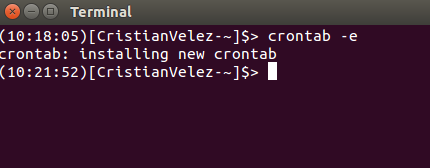
\includegraphics[scale=0.5]{pics/crontab2.png}  %el parámetro scale permite agrandar o achicar la imagen. En el nombre de archivo puede especificar directorios
	\caption{Creación crontab 2} \label{fig:figura2}
\end{figure}

Otra manera sería meter el script en la carpeta \textit{/etc/cron.daily/}, y cron \cite{cron} se encargará de ejecutarla diariamente.



%----------------------------------------------------------------------------------------
%	Cuestión 3
%----------------------------------------------------------------------------------------
\section[Cuestión 3]{ Pruebe a ejecutar el comando, conectar un dispositivo USB y vuelva a ejecutar el comando. Copie y pegue la salida del comando.(considere usar dmesg | tail). Comente qué observa en la información	mostrada.}

Si ejecutamos dmesg -T nos mostrará el log del kernel añadiendo la fecha y hora para poder ubicar mejor las cosas en el tiempo, lo que voy a hacer es hacer una llamada a dmesg -T y lo guardaré en un fichero, a continuación voy a introducir un pendrive, esperaré unos segundos y volveré a repetir el proceso pero guardándolo en otro fichero, para obtener lo que ha ocasionado el USB, bastará con hacer un diff entre los dos archivos .

Primero guardo en sinUSB la información antes de conectar el USB,

\begin{figure}[H] %con el [H] le obligamos a situar aquí la figura
	\centering
	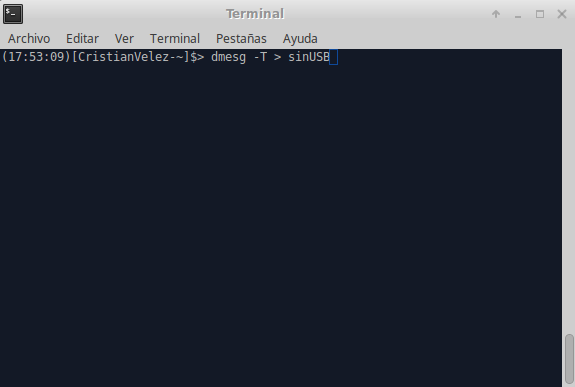
\includegraphics[scale=0.5]{pics/USB1.png}  %el parámetro scale permite agrandar o achicar la imagen. En el nombre de archivo puede especificar directorios
	\caption{Usb sin conectar} \label{fig:usb1}
\end{figure}

Conecto el USB y espero unos segundos, y vuelvo a repetir el proceso anterior cambiando el archivo a conUSB,

\begin{figure}[H] %con el [H] le obligamos a situar aquí la figura
	\centering
	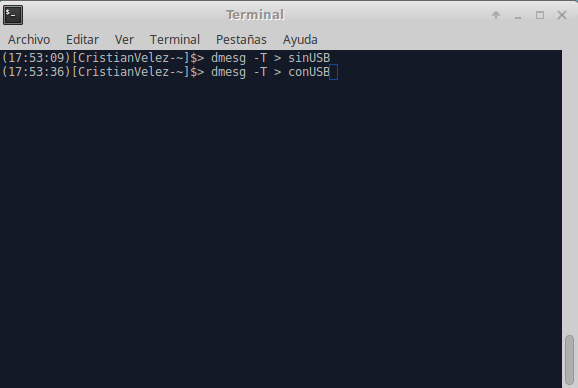
\includegraphics[scale=0.5]{pics/USB2.png}  %el parámetro scale permite agrandar o achicar la imagen. En el nombre de archivo puede especificar directorios
	\caption{Usb conectado} \label{fig:usb2}
\end{figure}

\begin{figure}[H] %con el [H] le obligamos a situar aquí la figura
	\centering
	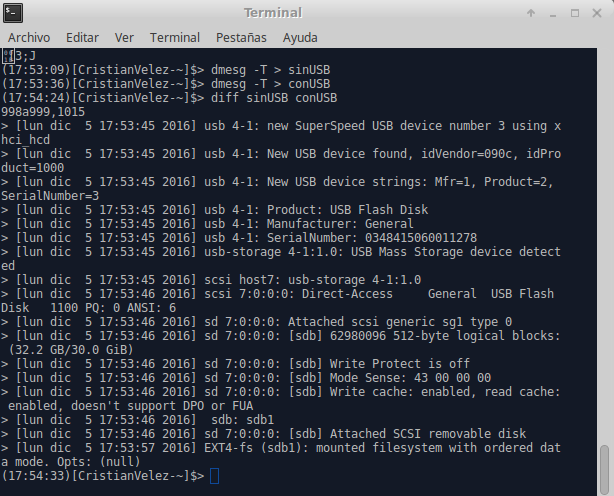
\includegraphics[scale=0.5]{pics/USB3.png}  %el parámetro scale permite agrandar o achicar la imagen. En el nombre de archivo puede especificar directorios
	\caption{Diferencias entre archivos} \label{fig:usb3}
\end{figure}

Como se puede ver detecta que es un pendrive 3.0, así como la identidad de su vendedor y el número de serie del producto, también comprueba si está protegido frente a escritura y es solo de lectura, detecta las particiones que tiene y finalmente monta las particiones.



%----------------------------------------------------------------------------------------
%	Cuestión 4
%----------------------------------------------------------------------------------------
\section[Cuestión 4]{Ejecute el monitor de “System Performance” y muestre el resultado. Incluya capturas de pantalla comentando la información que aparece.}

Para poder ejecutar perfmon \cite{perfmon}, lo primero que debemos hacer es llamarlo desde ejecutar.

\begin{figure}[H] %con el [H] le obligamos a situar aquí la figura
	\centering
	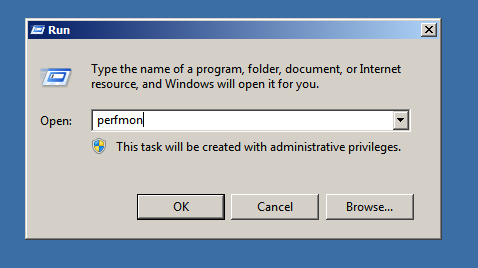
\includegraphics[scale=0.5]{pics/perfmon1.png}  %el parámetro scale permite agrandar o achicar la imagen. En el nombre de archivo puede especificar directorios
	\caption{Perfmon paso 1} \label{fig:perfmon1}
\end{figure}

Seguidamente ya nos saldrá la ventana del \textit{Perfomance Monitor}

\begin{figure}[H] %con el [H] le obligamos a situar aquí la figura
	\centering
	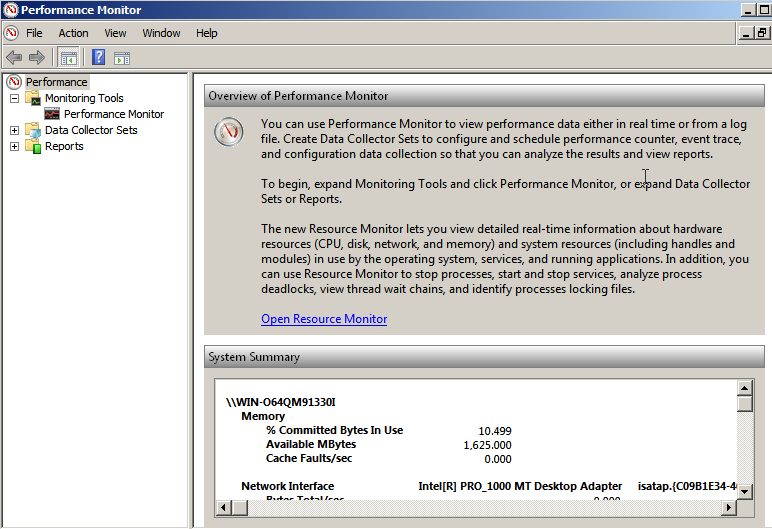
\includegraphics[scale=0.5]{pics/perfmon2.png}  %el parámetro scale permite agrandar o achicar la imagen. En el nombre de archivo puede especificar directorios
	\caption{Perfmon paso 2} \label{fig:perfmon2}
\end{figure}

Ahora lo que debemos hacer es ir a \textit{Data Colector Sets}, y buscamos \textit{System Performance}, pulsamos botón derecho encima y le damos a \textit{start}, ahora estará recopilando datos durante 60 s.

\begin{figure}[H] %con el [H] le obligamos a situar aquí la figura
	\centering
	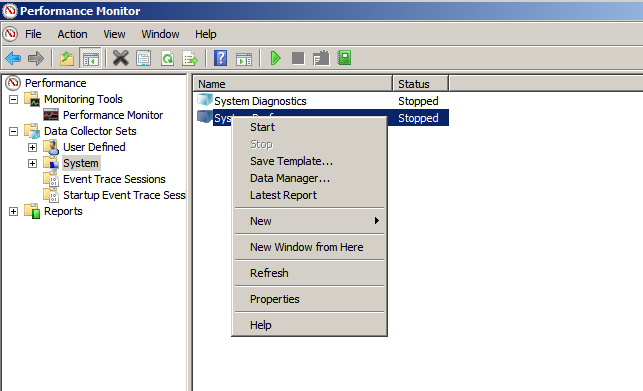
\includegraphics[scale=0.5]{pics/perfmon3.png}  %el parámetro scale permite agrandar o achicar la imagen. En el nombre de archivo puede especificar directorios
	\caption{Perfmon paso 3} \label{fig:perfmon3}
\end{figure}

Si vamos a \textit{reports}, podemos apreciar que está recopilando datos,

\begin{figure}[H] %con el [H] le obligamos a situar aquí la figura
	\centering
	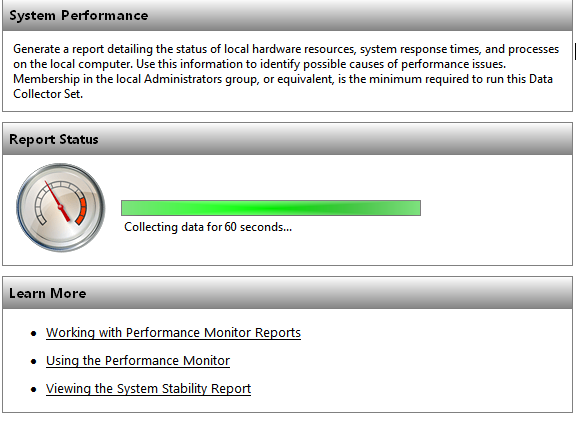
\includegraphics[scale=0.5]{pics/perfmon4.png}  %el parámetro scale permite agrandar o achicar la imagen. En el nombre de archivo puede especificar directorios
	\caption{Perfmon paso 4} \label{fig:perfmon4}
\end{figure}

Una vez ha terminado nos muestra la información que ha estado recopilando, nos muestra cuando se ejecutó el recopilador, y la información relativa al equipo donde se lanzó.

\begin{figure}[H] %con el [H] le obligamos a situar aquí la figura
	\centering
	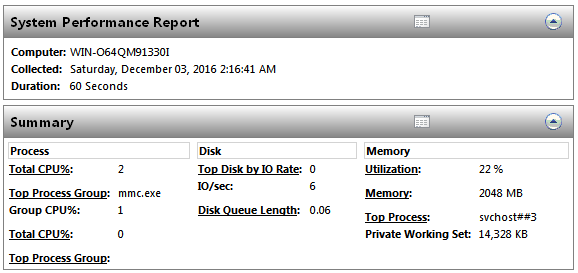
\includegraphics[scale=0.5]{pics/perfmon5.png}  %el parámetro scale permite agrandar o achicar la imagen. En el nombre de archivo puede especificar directorios
	\caption{Perfmon paso 5} \label{fig:perfmon5}
\end{figure}

En esta segunda foto se puede apreciar que nos hace un resumen de la carga de la CPU, red, discos y memoria ram.

\begin{figure}[H] %con el [H] le obligamos a situar aquí la figura
	\centering
	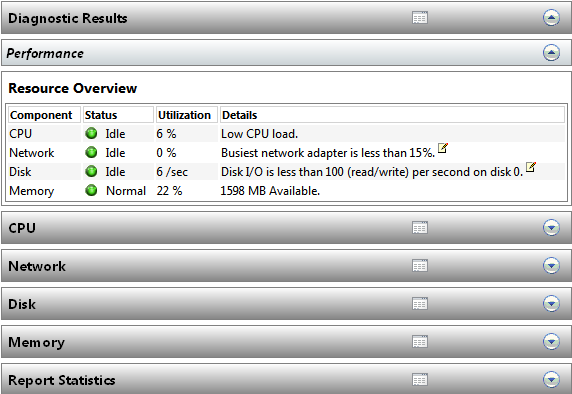
\includegraphics[scale=0.5]{pics/perfmon6.png}  %el parámetro scale permite agrandar o achicar la imagen. En el nombre de archivo puede especificar directorios
	\caption{Perfmon paso 6} \label{fig:perfmon6}
\end{figure}

Toda esta información se puede ver más detallada en las pestañas de abajo, tales como procesos que se han ejecutado, qué servicios consumían más recursos, qué servicio usó la red y un largo etcétera









%----------------------------------------------------------------------------------------
%	Cuestión 5
%----------------------------------------------------------------------------------------
\section[Cuestión 5]{ Cree un recopilador de datos definido por el usuario (modo avanzado) que incluya tanto el contador de rendimiento como los datos de seguimiento:
	Todos los referentes al procesador, al proceso y al servicio web, 
	Intervalo de muestra 15 segundos, 
	Almacene el resultado en el directorio Escritorio/logs, 
	Incluya las capturas de pantalla de cada paso.}

Lo primero que debemos hacer es dar botón derecho sobre \textit{user defined}, y le damos a new Data \textit{Collector Sets}

\begin{figure}[H] %con el [H] le obligamos a situar aquí la figura
	\centering
	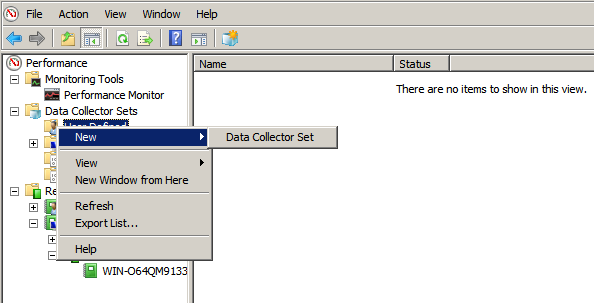
\includegraphics[scale=0.5]{pics/recopilador1.png}  %el parámetro scale permite agrandar o achicar la imagen. En el nombre de archivo puede especificar directorios
	\caption{Recopilador paso 1} \label{fig:reco1}
\end{figure}

Seleccionamos el nombre que le queremos poner y la opción de modo avanzado.
\begin{figure}[H] %con el [H] le obligamos a situar aquí la figura
	\centering
	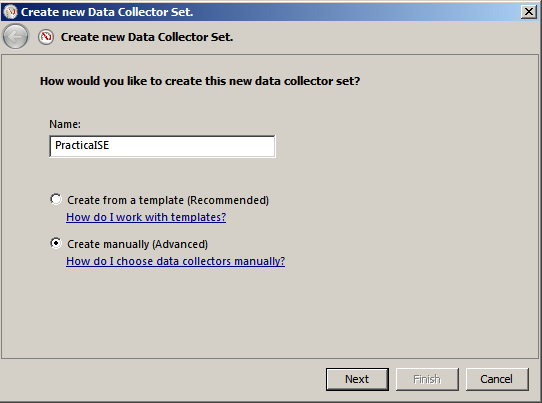
\includegraphics[scale=0.5]{pics/recopilador2.png}  %el parámetro scale permite agrandar o achicar la imagen. En el nombre de archivo puede especificar directorios
	\caption{Recopilador paso 2} \label{fig:reco2}
\end{figure}

Ahora debemos seleccionar \textit{Performance Counter} y \textit{Events trace data} y le damos a siguiente.

\begin{figure}[H] %con el [H] le obligamos a situar aquí la figura
	\centering
	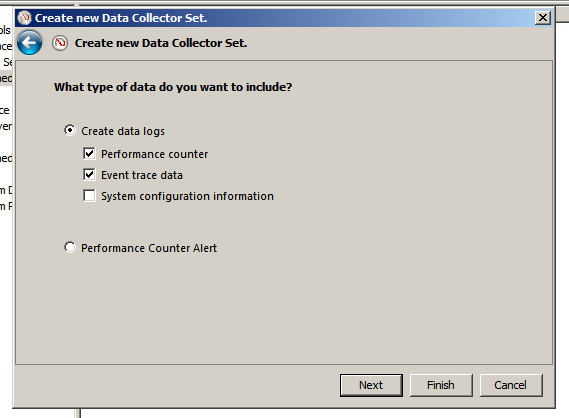
\includegraphics[scale=0.5]{pics/recopilador3.png}  %el parámetro scale permite agrandar o achicar la imagen. En el nombre de archivo puede especificar directorios
	\caption{Recopilador paso 3} \label{fig:reco3}
\end{figure}

En este paso debemos seleccionar que queremos que nos monitorice, yo he seleccionado \textit{Proccess, Processor, Processor Information e IIS Global}, para que monitorice el procesador, los procesos e IIS.
\begin{figure}[H] %con el [H] le obligamos a situar aquí la figura
	\centering
	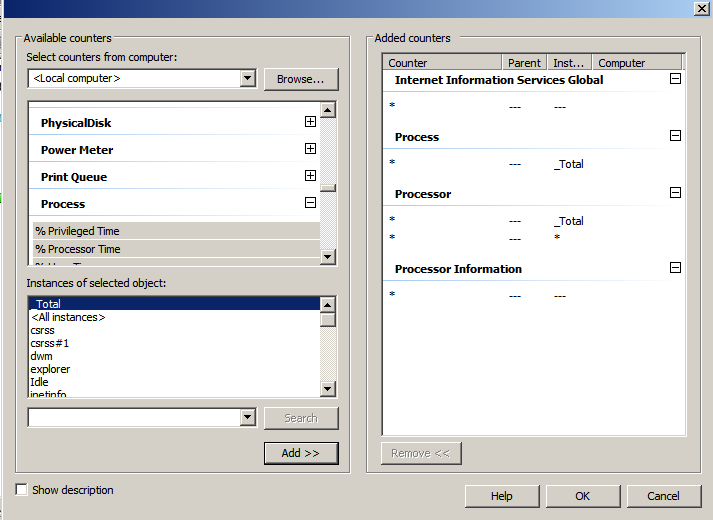
\includegraphics[scale=0.5]{pics/recopilador4.png}  %el parámetro scale permite agrandar o achicar la imagen. En el nombre de archivo puede especificar directorios
	\caption{Recopilador paso 4} \label{fig:reco4}
\end{figure}

Seleccionamos cada cuánto tiempo queremos que haga un muestreo, en nuestro caso 15 segundos y damos a next.

\begin{figure}[H] %con el [H] le obligamos a situar aquí la figura
	\centering
	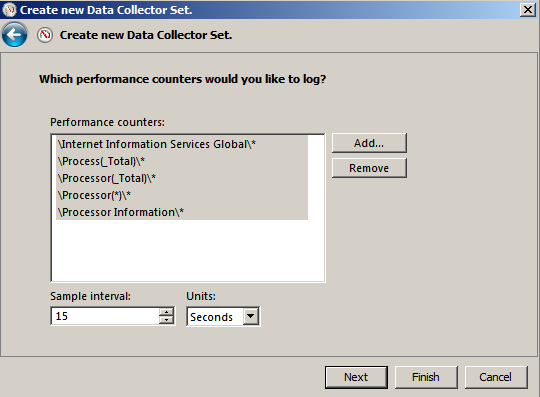
\includegraphics[scale=0.5]{pics/recopilador5.png}  %el parámetro scale permite agrandar o achicar la imagen. En el nombre de archivo puede especificar directorios
	\caption{Recopilador paso 5} \label{fig:reco5}
\end{figure}

Debemos seleccionar los eventos que queremos muestrear, ahora seleccionaremos los que tengan que ver con IIS.
\begin{figure}[H] %con el [H] le obligamos a situar aquí la figura
	\centering
	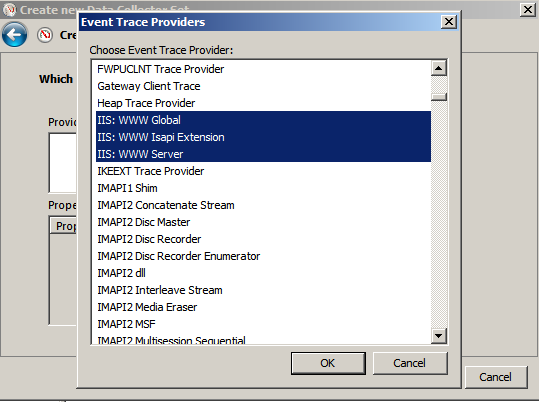
\includegraphics[scale=0.5]{pics/recopilador6.png}  %el parámetro scale permite agrandar o achicar la imagen. En el nombre de archivo puede especificar directorios
	\caption{Recopilador paso 6} \label{fig:reco6}
\end{figure}

Definimos donde queremos que se guarden los datos del recopilador: \textit{Escritorio/Logs}
\begin{figure}[H] %con el [H] le obligamos a situar aquí la figura
	\centering
	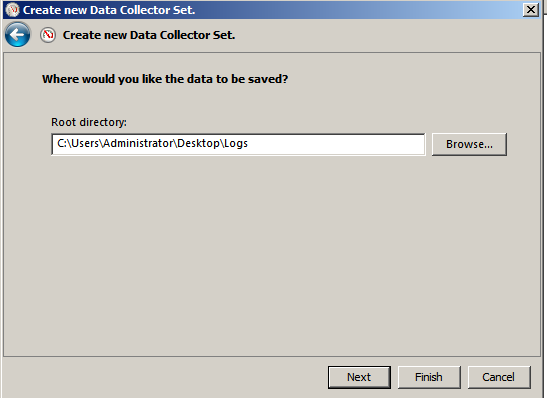
\includegraphics[scale=0.5]{pics/recopilador7.png}  %el parámetro scale permite agrandar o achicar la imagen. En el nombre de archivo puede especificar directorios
	\caption{Recopilador paso 7} \label{fig:reco7}
\end{figure}

Y finalmente damos en finish.

\begin{figure}[H] %con el [H] le obligamos a situar aquí la figura
	\centering
	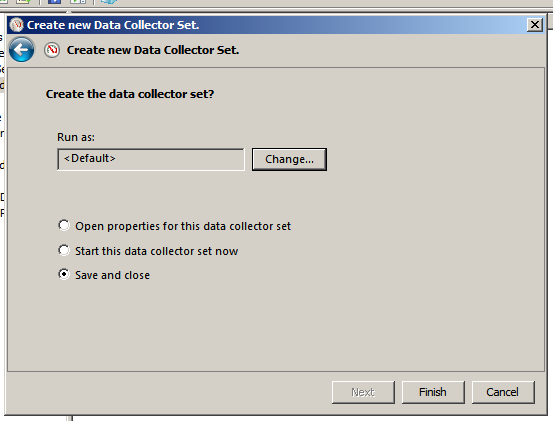
\includegraphics[scale=0.5]{pics/recopilador8.png}  %el parámetro scale permite agrandar o achicar la imagen. En el nombre de archivo puede especificar directorios
	\caption{Recopilador paso 8} \label{fig:reco8}
\end{figure}

Vamos a ejecutar nuestro recopilador, damos a \textit{start}
\begin{figure}[H] %con el [H] le obligamos a situar aquí la figura
	\centering
	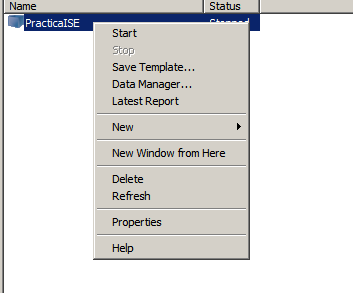
\includegraphics[scale=0.5]{pics/recopilador9.png}  %el parámetro scale permite agrandar o achicar la imagen. En el nombre de archivo puede especificar directorios
	\caption{Recopilador paso 9} \label{fig:reco9}
\end{figure}

Ahora estará recopilando datos cada 15 segundos hasta que lo paremos.
\begin{figure}[H] %con el [H] le obligamos a situar aquí la figura
	\centering
	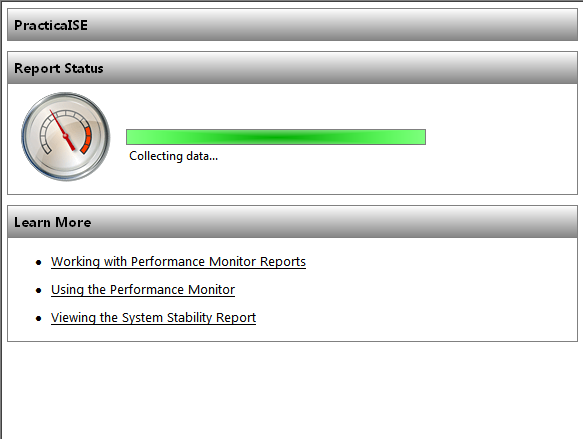
\includegraphics[scale=0.5]{pics/recopilador10.png}  %el parámetro scale permite agrandar o achicar la imagen. En el nombre de archivo puede especificar directorios
	\caption{Recopilador paso 10} \label{fig:reco10}
\end{figure}

Si vamos a nuestro escritorio podemos observar la carpeta que nos ha generado, así como los datos que ha recopilado.

\begin{figure}[H] %con el [H] le obligamos a situar aquí la figura
	\centering
	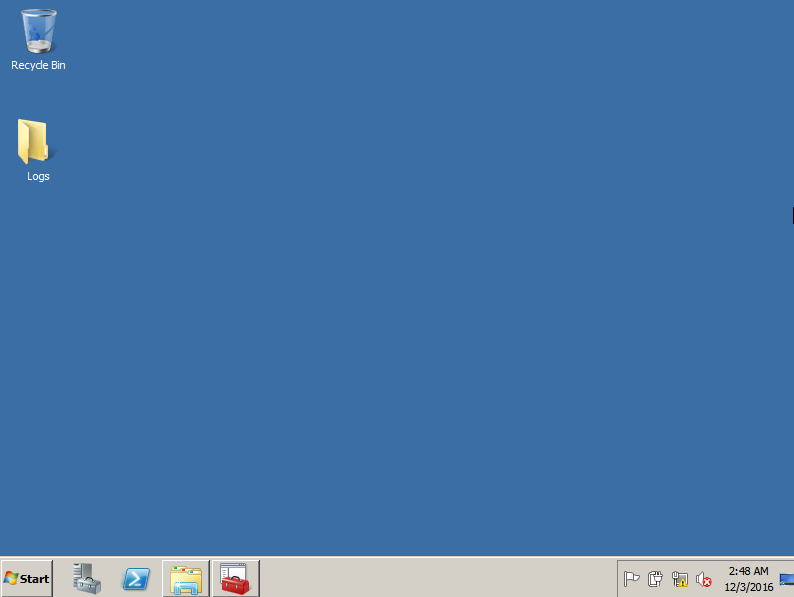
\includegraphics[scale=0.5]{pics/recopilador11.png}  %el parámetro scale permite agrandar o achicar la imagen. En el nombre de archivo puede especificar directorios
	\caption{Recopilador paso 11} \label{fig:reco11}
\end{figure}

\begin{figure}[H] %con el [H] le obligamos a situar aquí la figura
	\centering
	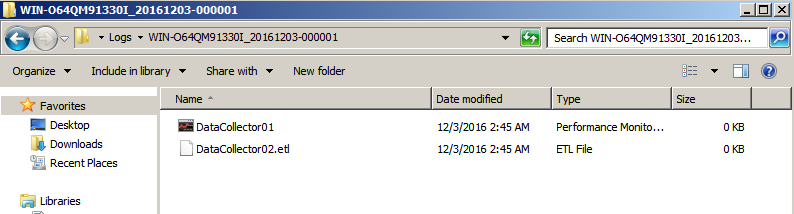
\includegraphics[scale=0.5]{pics/recopilador12.png}  %el parámetro scale permite agrandar o achicar la imagen. En el nombre de archivo puede especificar directorios
	\caption{Recopilador paso 12} \label{fig:reco12}
\end{figure}

Vamos a inspeccionar los datos de DataCollector01, damos doble click y se nos abre.

\begin{figure}[H] %con el [H] le obligamos a situar aquí la figura
	\centering
	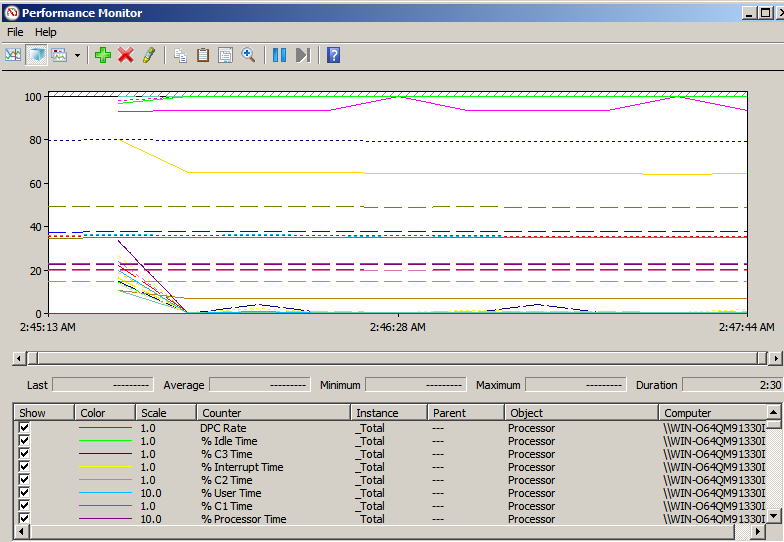
\includegraphics[scale=0.5]{pics/recopilador13.png}  %el parámetro scale permite agrandar o achicar la imagen. En el nombre de archivo puede especificar directorios
	\caption{Recopilador paso 13} \label{fig:reco13}
\end{figure}

Ya tenemos nuestro recopilador funcionando. \cite{crear}

%----------------------------------------------------------------------------------------
%	Cuestión 6
%----------------------------------------------------------------------------------------
\section[Cuestión 6]{Visite la web del proyecto y acceda a la demo que proporcionan (http://demo.munin-monitoring.org/) donde se muestra cómo	monitorizan un servidor. Monitorice varios parámetros y haga capturas de pantalla de lo que está mostrando comentando qué observa.}

Accedemos a la página de la demo de Munin \cite{munim} y lo que nos encontramos nada mas entrar es 

\begin{figure}[H] %con el [H] le obligamos a situar aquí la figura
	\centering
	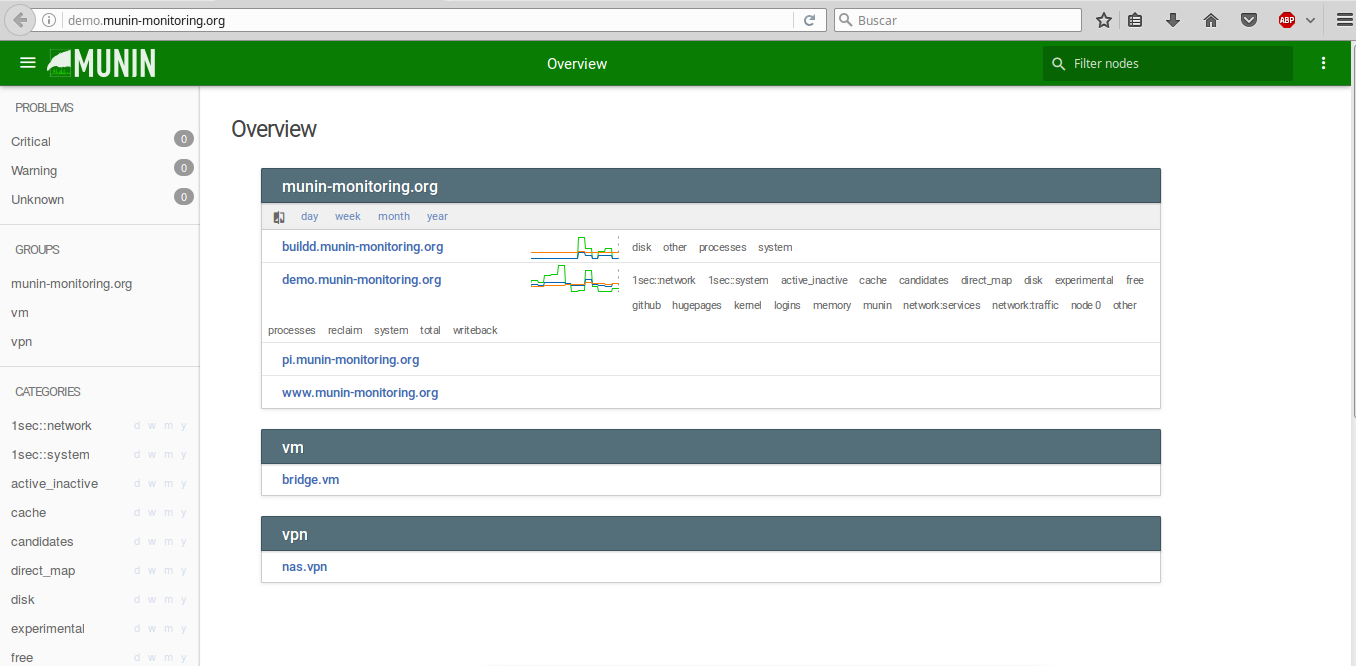
\includegraphics[scale=0.35]{pics/munin1.png}  %el parámetro scale permite agrandar o achicar la imagen. En el nombre de archivo puede especificar directorios
	\caption{Munin 1} \label{fig:munin1}
\end{figure}

Seleccionamos el segundo que es lo que más está monitorizando, y vamos a visualizar \textit{disk}

\begin{figure}[H] %con el [H] le obligamos a situar aquí la figura
	\centering
	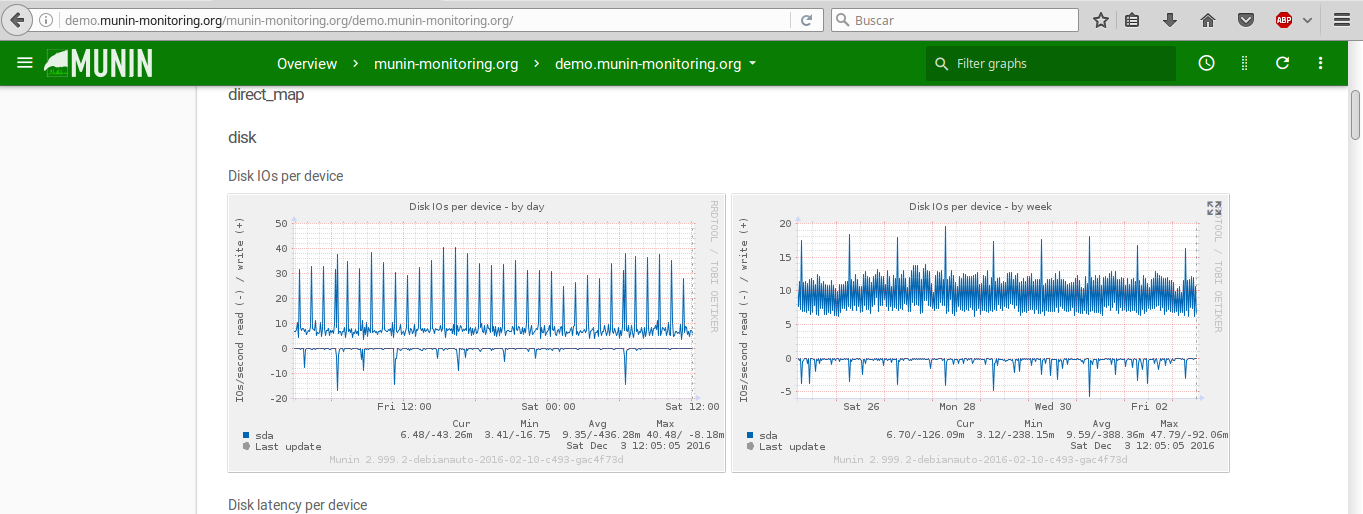
\includegraphics[scale=0.35]{pics/munin2.png}  %el parámetro scale permite agrandar o achicar la imagen. En el nombre de archivo puede especificar directorios
	\caption{Munin 2} \label{fig:munin2}
\end{figure}

Pinchamos y nos muestra 4 gráficas, en una está lo que ha monitorizado durante el día, otra durante la semana,mes y año.\\

Como se puede apreciar en la gráfica de día, es evidente cuando realizan más operaciones en disco, así como cuando menos se utiliza el disco, que es el sábado a las 1:00.


\begin{figure}[H] %con el [H] le obligamos a situar aquí la figura
	\centering
	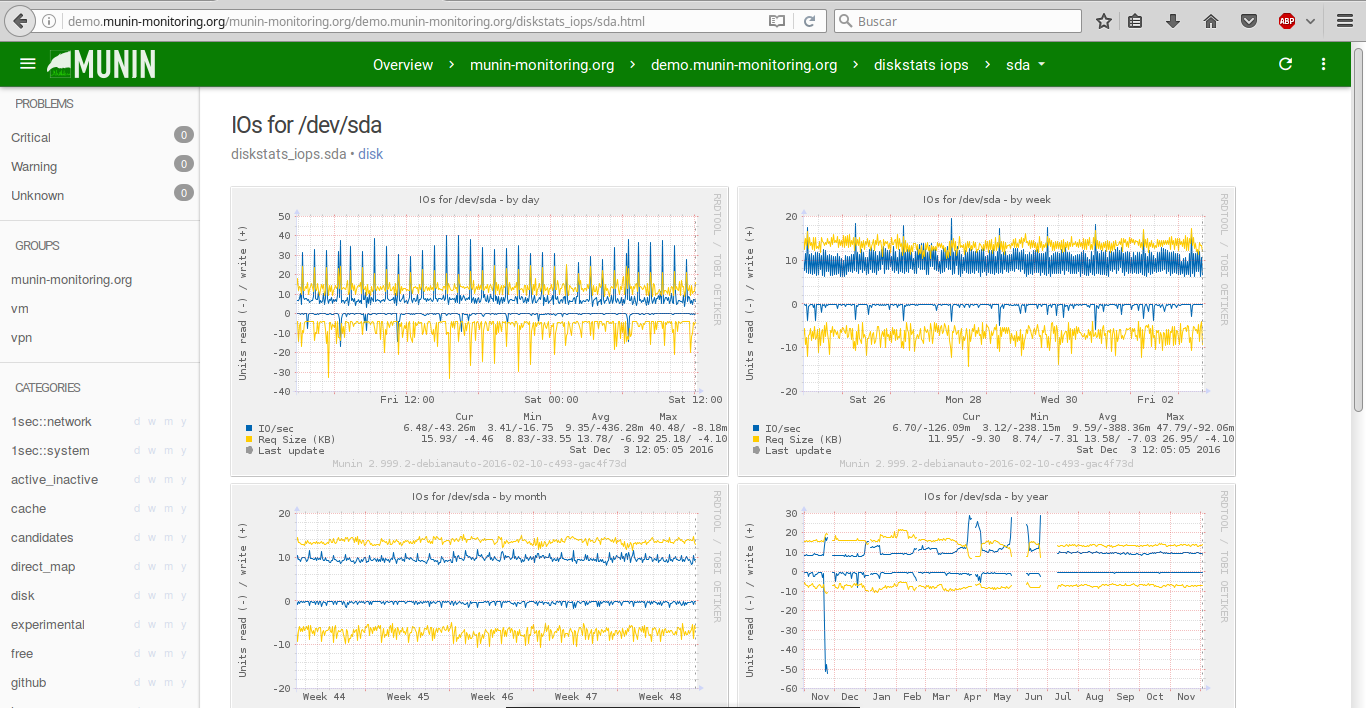
\includegraphics[scale=0.35]{pics/munin3.png}  %el parámetro scale permite agrandar o achicar la imagen. En el nombre de archivo puede especificar directorios
	\caption{Munin 3} \label{fig:munin3}
\end{figure}

Al igual que con el uso de disco vamos a inspeccionar la red,

\begin{figure}[H] %con el [H] le obligamos a situar aquí la figura
	\centering
	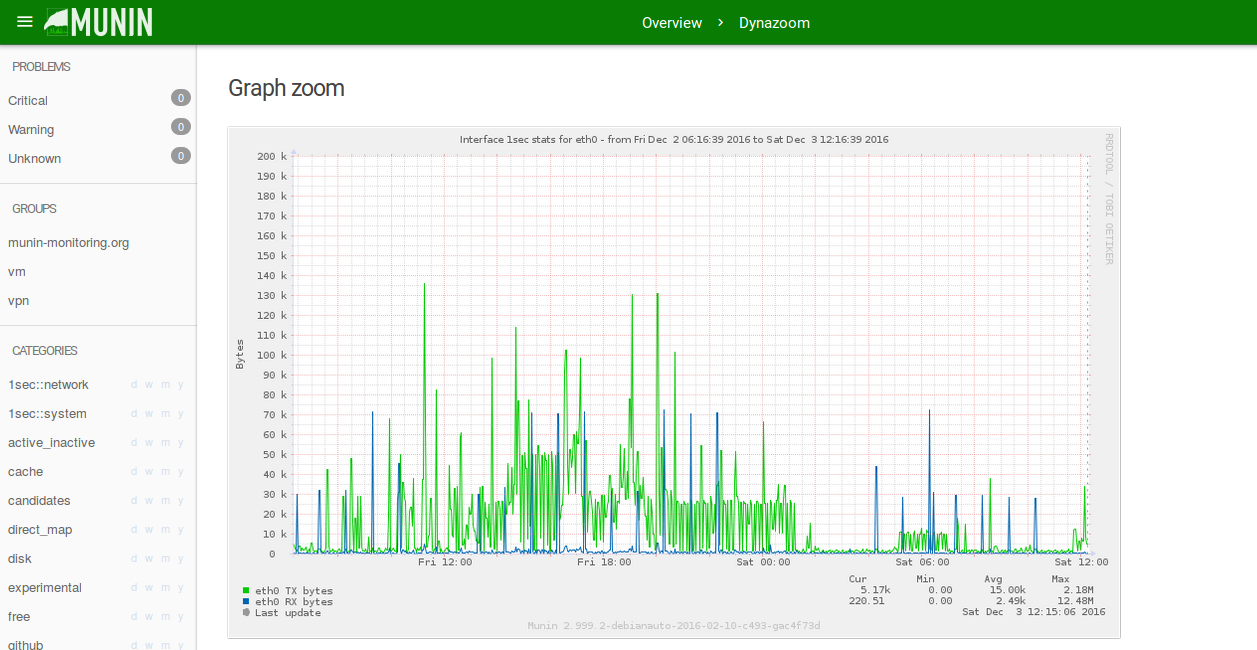
\includegraphics[scale=0.35]{pics/munin4.png}  %el parámetro scale permite agrandar o achicar la imagen. En el nombre de archivo puede especificar directorios
	\caption{Munin 4} \label{fig:munin4}
\end{figure}

También al igual que los discos, se puede apreciar que cuando menos actividad de red  tiene coincide con el mismo punto que los discos, lo que nos quiere decir que es cuando el sistema apenas se esta utilizando, ya que la red apenas tiene tráfico.

%----------------------------------------------------------------------------------------
%	Cuestión 7
%----------------------------------------------------------------------------------------
\section[Cuestión 7]{ Escriba un breve resumen sobre alguno de los artículos donde se muestra el uso de strace o busque otro y coméntelo.}

Strace es una herramienta en línea de comando que sirve para poder visualizar las llamadas al sistema que realiza un determinado programa, así como ver cuantos threads lanza para su ejecución, podemos obtener estadísticas de el número de llamadas al sistema que ha realizado, el porcentaje de ejecución que ha consumido ese tipo de llamada y así como el numero de errores de cada una de ellas.\\
\\
Strace es una buena herramienta para poder detectar que ocurre entre nuestro programa y el sistema, si algo parece que no debe ir bien.

%----------------------------------------------------------------------------------------
%	Cuestión 8
%----------------------------------------------------------------------------------------
\section[Cuestión 8]{ Escriba un script en Python o PHP y analice su comportamiento usando el profiler presentado.}

Mi script está realizado en python3 \cite{python}, genero dos matrices con números aleatorios, y luego creo una última con la multiplicación de las posiciones anteriores, sol(i,j)=a(i,j)*b(i,j)

\begin{lstlisting}[language=python]
import random

filas = 1000
columnas = 1000

matrizA= []
for i in range(filas):
	matrizA.append([])
	for j in range(columnas):
		matrizA[i].append(random.randint(0,100))

matrizB= []
for i in range(filas):
	matrizB.append([])
	for j in range(columnas):
		matrizB[i].append(random.randint(0,100))



matrizSol=[]
for i in range(filas):
	matrizSol.append([])
	for j in range(columnas):
		matrizSol[i].append((matrizA[i][j]*matrizB[i][j]))


print(matrizSol)
\end{lstlisting}

Ahora básicamente lo que haré sera ejecutarlo con el profiler de python3 mediante \textit{python3 -m cProfile -o salida script.py},

\begin{figure}[H] %con el [H] le obligamos a situar aquí la figura
	\centering
	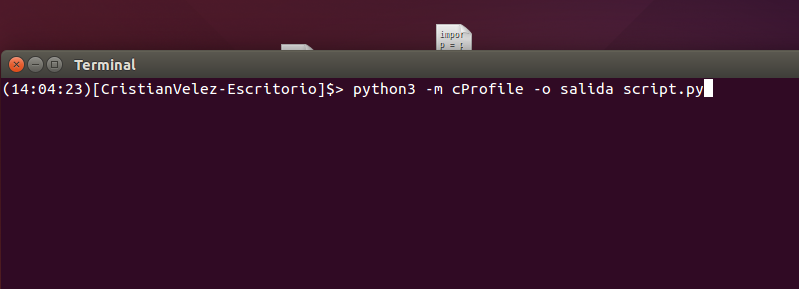
\includegraphics[scale=0.35]{pics/python1.png}  %el parámetro scale permite agrandar o achicar la imagen. En el nombre de archivo puede especificar directorios
	\caption{Python 1} \label{fig:python1}
\end{figure}

\begin{figure}[H] %con el [H] le obligamos a situar aquí la figura
	\centering
	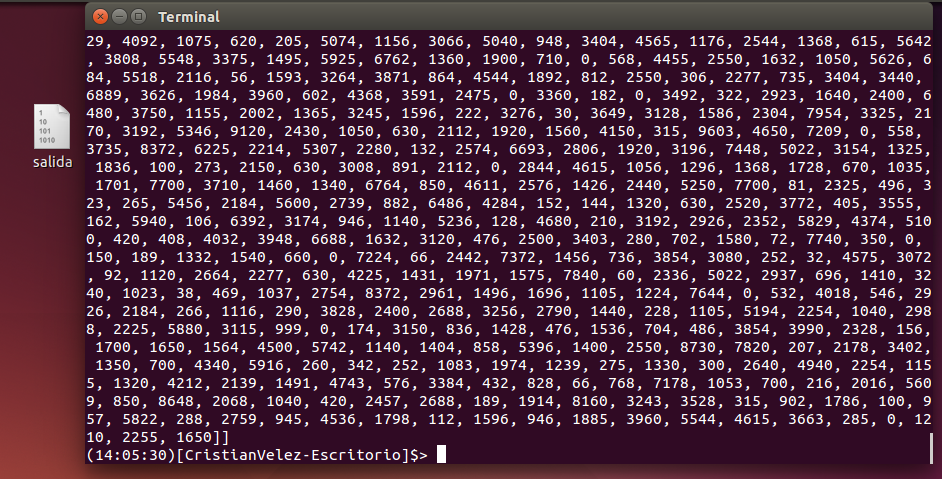
\includegraphics[scale=0.35]{pics/python2.png}  %el parámetro scale permite agrandar o achicar la imagen. En el nombre de archivo puede especificar directorios
	\caption{Python 2} \label{fig:python2}
\end{figure}

Ahora nos ha generado un archivo que no es legible llamado salida, para poder visualizarlo crearemos otro pequeño script que nos mostrará las estadísticas legibles,


\begin{lstlisting}[language=python]
import pstats

p = pstats.Stats('salida')
p.strip_dirs().sort_stats(-1).print_stats()
\end{lstlisting}


\begin{figure}[H] %con el [H] le obligamos a situar aquí la figura
	\centering
	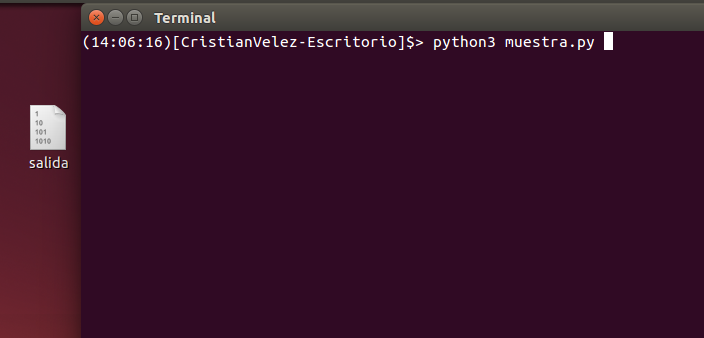
\includegraphics[scale=0.35]{pics/python3.png}  %el parámetro scale permite agrandar o achicar la imagen. En el nombre de archivo puede especificar directorios
	\caption{Python 3} \label{fig:python3}
\end{figure}

Como se puede apreciar nos muestra todas las llamadas que ha generado el script,

\begin{figure}[H] %con el [H] le obligamos a situar aquí la figura
	\centering
	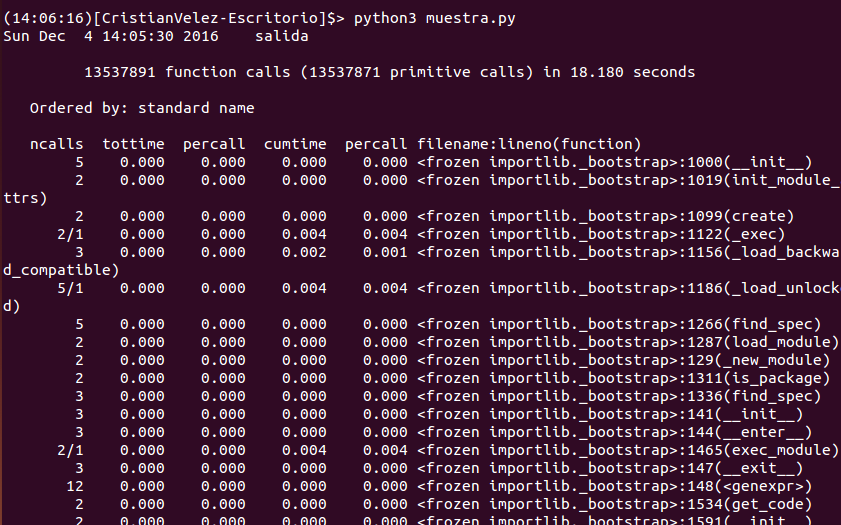
\includegraphics[scale=0.35]{pics/python4.png}  %el parámetro scale permite agrandar o achicar la imagen. En el nombre de archivo puede especificar directorios
	\caption{Python 4} \label{fig:python4}
\end{figure}

Aquí podemos apreciar las llamadas a random que ha usado para poder generar los números aleatorios de las matrices así como inicializar la semilla una vez y luego 2.000.000 de llamadas a random y como era de esperar es el número de aleatorios que generamos, 1000x1000 = 1.000.000 cada matriz, si tenemos dos sería 2.000.000 de números aleatorios en total.

\begin{figure}[H] %con el [H] le obligamos a situar aquí la figura
	\centering
	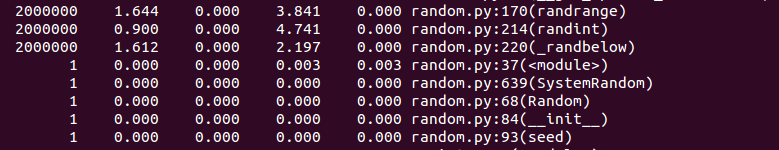
\includegraphics[scale=0.35]{pics/python5.png}  %el parámetro scale permite agrandar o achicar la imagen. En el nombre de archivo puede especificar directorios
	\caption{Python 5} \label{fig:python5}
\end{figure}





%----------------------------------------------------------------------------------------
%	Cuestión 9
%----------------------------------------------------------------------------------------
\section[Cuestión 9]{   Acceda a la consola mysql (o a través de phpMyAdmin) y	muestre el resultado de mostrar el ”profile” de una consulta (la creación de la BD y la consulta la puede hacer libremente).}

Primero lo que voy a hacer es acceder a mysql \cite{mysql} desde la terminal, 

\begin{figure}[H] %con el [H] le obligamos a situar aquí la figura
	\centering
	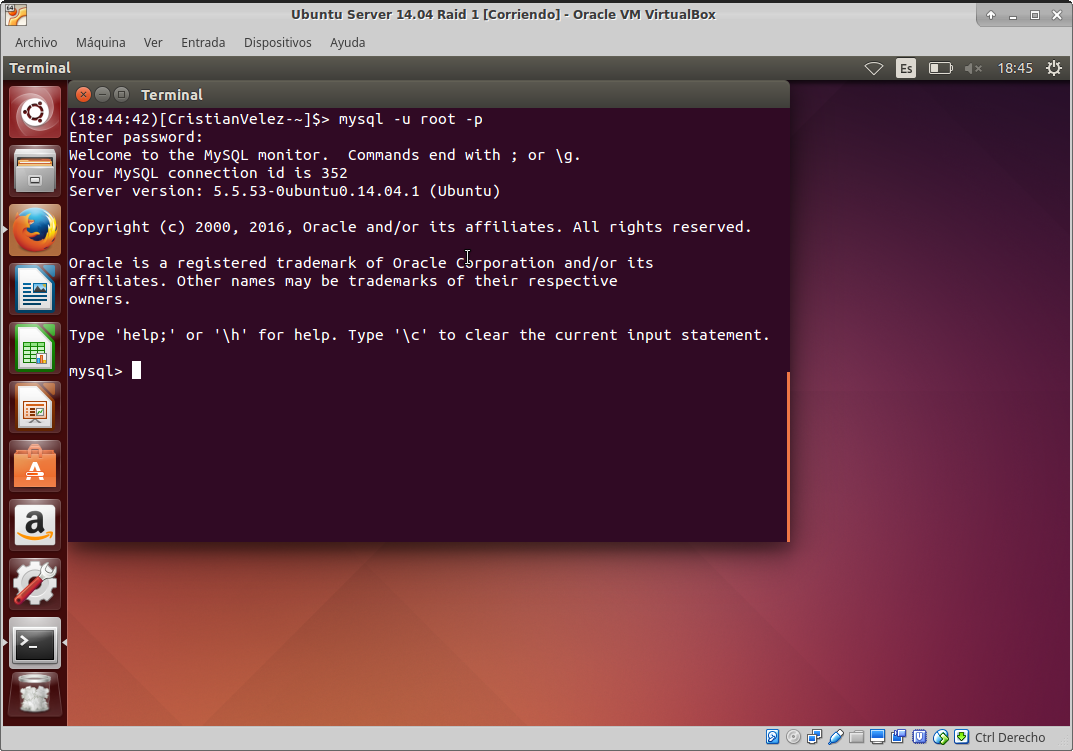
\includegraphics[scale=0.35]{pics/profile1.png}  %el parámetro scale permite agrandar o achicar la imagen. En el nombre de archivo puede especificar directorios
	\caption{Profiler mysql 1} \label{fig:p1}
\end{figure}

Una vez estamos dentro vamos a decirle a mysql que base de datos queremos utilizar para ello usaremos \textit{USE mysql;}

\begin{figure}[H] %con el [H] le obligamos a situar aquí la figura
	\centering
	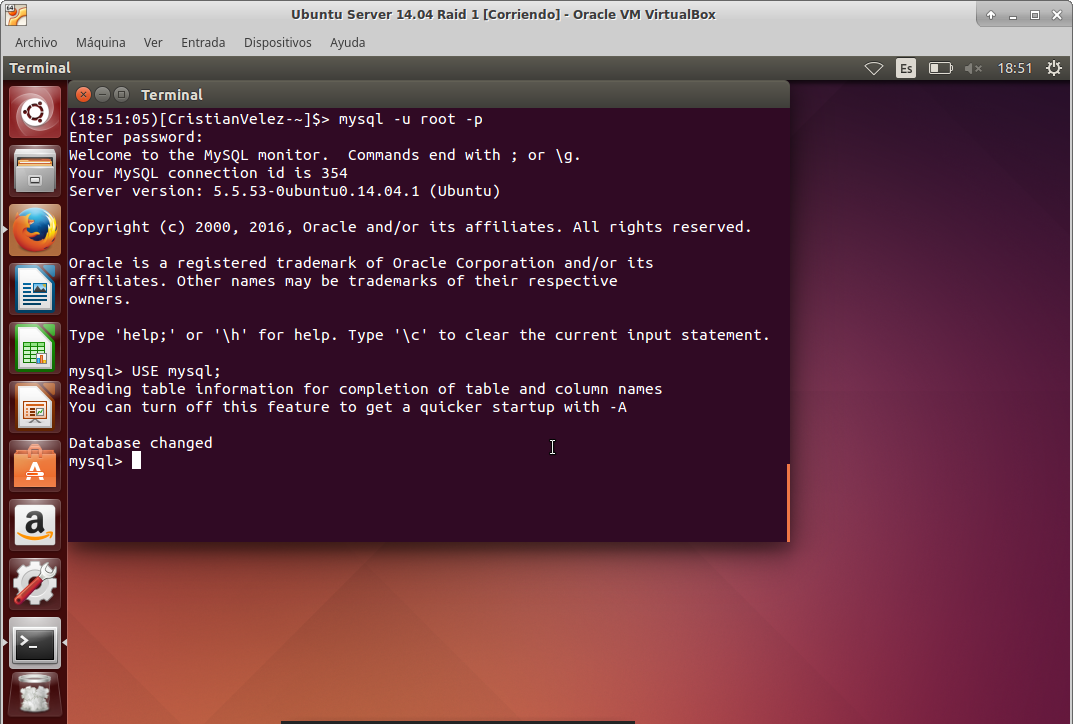
\includegraphics[scale=0.35]{pics/profile2.png}  %el parámetro scale permite agrandar o achicar la imagen. En el nombre de archivo puede especificar directorios
	\caption{Profiler mysql 2} \label{fig:p2}
\end{figure}

Ahora debemos activar el profiling , con \textit{SET profiling=1;}, lo que hagamos a partir de ahora quedará registrado su tiempo y estadística de cada operación que realicemos.

\begin{figure}[H] %con el [H] le obligamos a situar aquí la figura
	\centering
	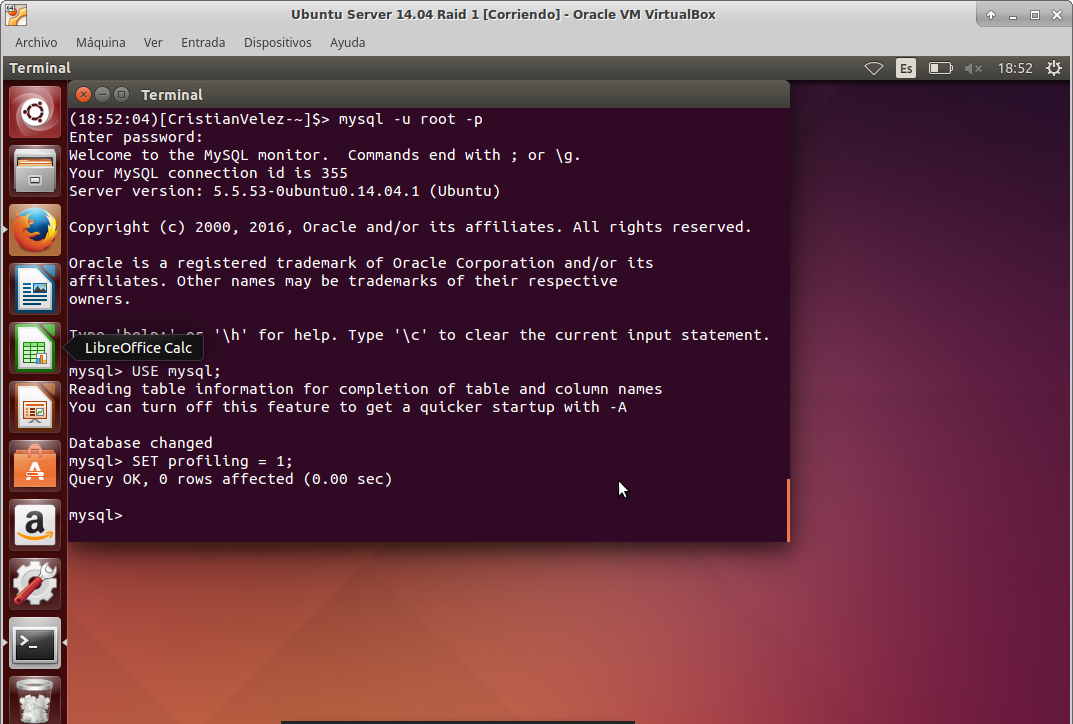
\includegraphics[scale=0.35]{pics/profile3.png}  %el parámetro scale permite agrandar o achicar la imagen. En el nombre de archivo puede especificar directorios
	\caption{Profiler mysql 3} \label{fig:p3}
\end{figure}

Intentamos crear una tabla alumnos, pero como anteriormente fue creada como prueba da error.

\begin{figure}[H] %con el [H] le obligamos a situar aquí la figura
	\centering
	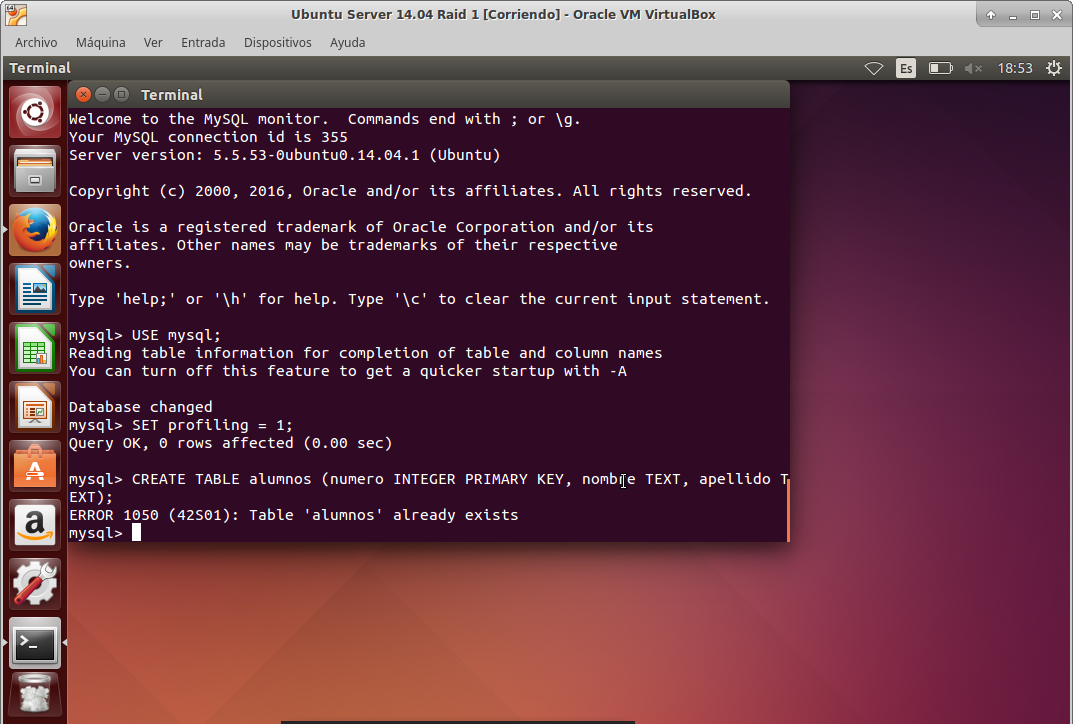
\includegraphics[scale=0.35]{pics/profile4.png}  %el parámetro scale permite agrandar o achicar la imagen. En el nombre de archivo puede especificar directorios
	\caption{Profiler mysql 4} \label{fig:p4}
\end{figure}

Eliminamos la tabla anterior con \textit{DROP alumnos;} y creamos una nueva de la misma manera que se intentó anteriormente.

\begin{figure}[H] %con el [H] le obligamos a situar aquí la figura
	\centering
	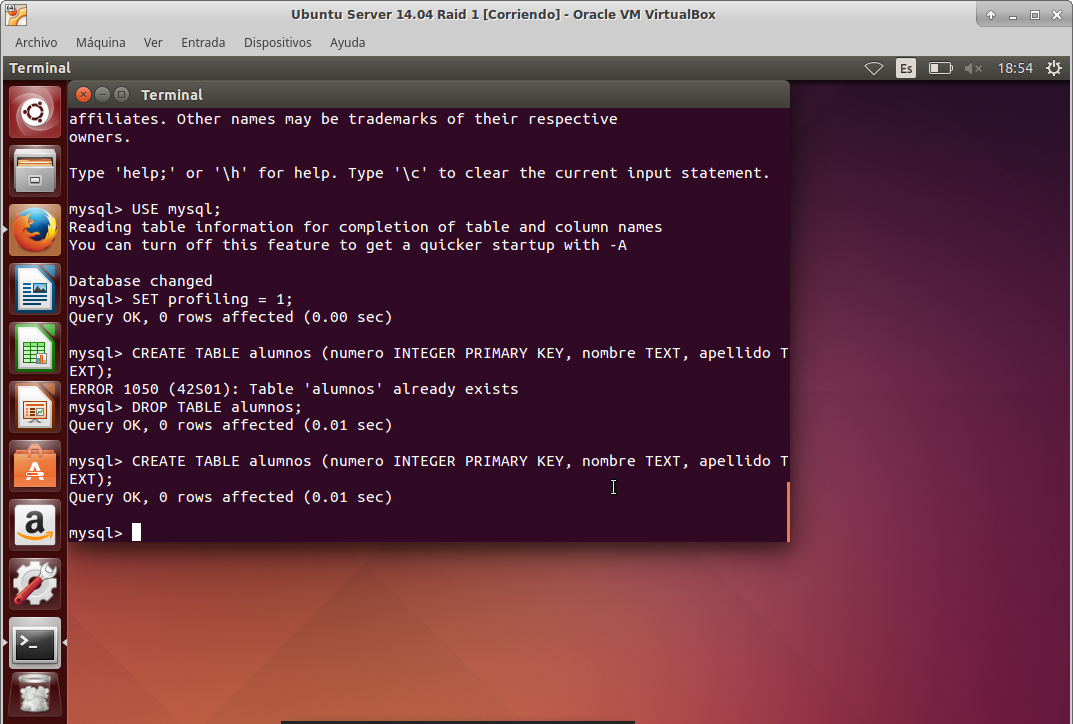
\includegraphics[scale=0.35]{pics/profile5.png}  %el parámetro scale permite agrandar o achicar la imagen. En el nombre de archivo puede especificar directorios
	\caption{Profiler mysql 5} \label{fig:p5}
\end{figure}

Ahora voy a insertar los datos de los alumnos para poder realizar una consulta.

\begin{figure}[H] %con el [H] le obligamos a situar aquí la figura
	\centering
	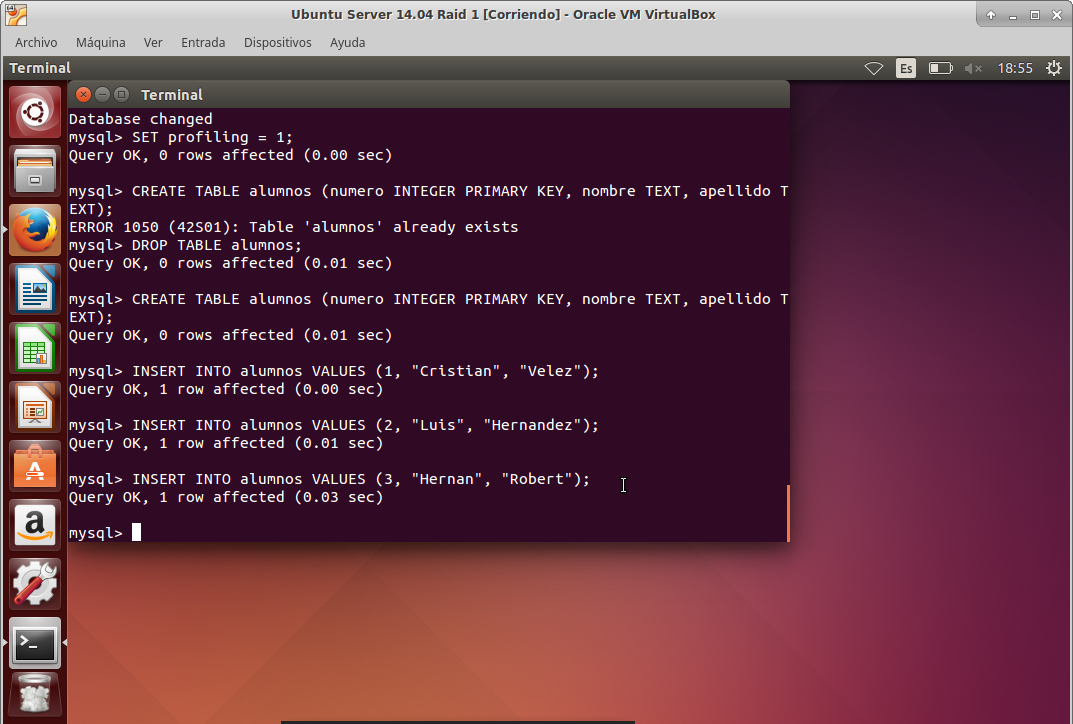
\includegraphics[scale=0.35]{pics/profile6.png}  %el parámetro scale permite agrandar o achicar la imagen. En el nombre de archivo puede especificar directorios
	\caption{Profiler mysql 6} \label{fig:p6}
\end{figure}

Una vez ya está rellena la tabla, voy a hacer una consulta para ver si obtengo como me llamo a partir de mi apellido con \textit{SELECT nombre FROM alumnos WHERE apellido="Velez";}

\begin{figure}[H] %con el [H] le obligamos a situar aquí la figura
	\centering
	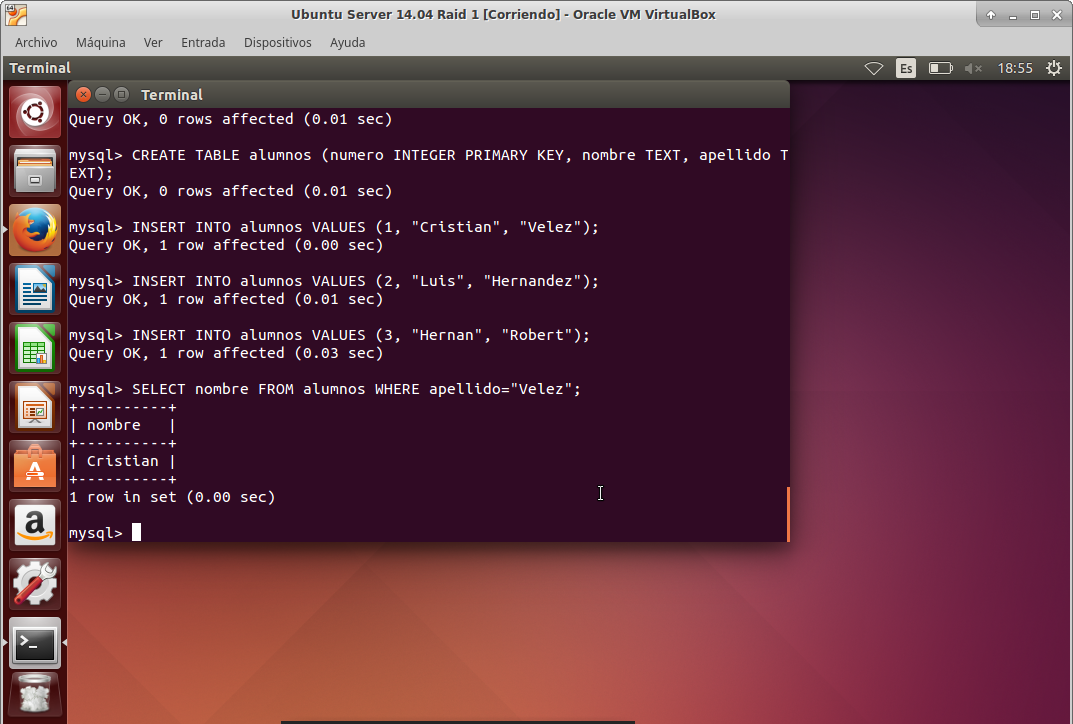
\includegraphics[scale=0.35]{pics/profile7.png}  %el parámetro scale permite agrandar o achicar la imagen. En el nombre de archivo puede especificar directorios
	\caption{Profiler mysql 7} \label{fig:p7}
\end{figure}

Una vez terminadas las operaciones vamos a ver lo que ha registrado el profiler de mysql, para ello basta con \textit{SHOW PROFILES;}

\begin{figure}[H] %con el [H] le obligamos a situar aquí la figura
	\centering
	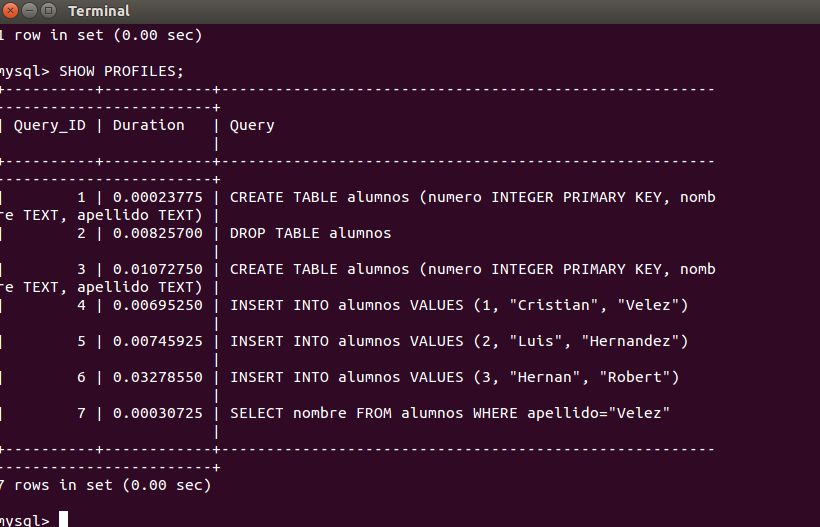
\includegraphics[scale=0.35]{pics/profile8.png}  %el parámetro scale permite agrandar o achicar la imagen. En el nombre de archivo puede especificar directorios
	\caption{Profiler mysql 8} \label{fig:p8}
\end{figure}

Ya podemos ver el tiempo que nos ha tardado en cada una de las operaciones y ver cuales pueden ser más costosas para nuestro sistema, en mi caso ha sido al crear la tabla alumnos.


\bibliography{citas} %archivo citas.bib que contiene las entradas 
\bibliographystyle{plain} % hay varias formas de citar

\end{document}
\grid
